\subsection{Optimal $hp$ combination}
\begin{figure}[h!]
    \centering
    % First row of subfigures (3 subfigures)
    \begin{subfigure}[t]{0.45\textwidth}
        \centering
        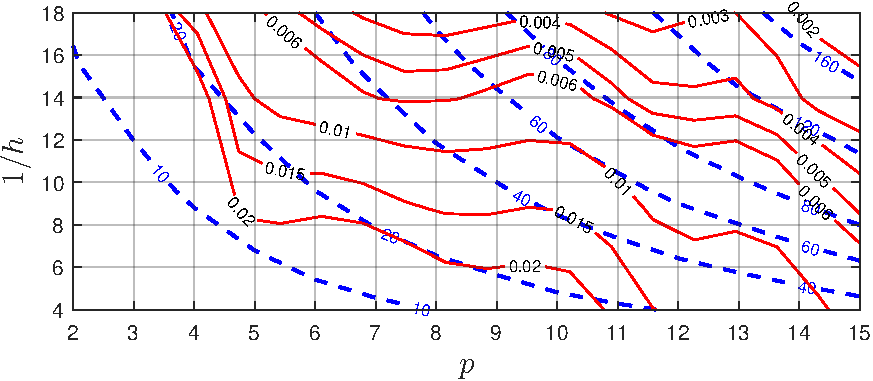
\includegraphics[width=\linewidth, height=4cm]{figs/hp_str-quad.pdf}  
        \caption{structured quadrilateral mesh}
        \label{hp_str-quad}
    \end{subfigure}
    %\hfill
    \begin{subfigure}[t]{0.45\textwidth}
        \centering
        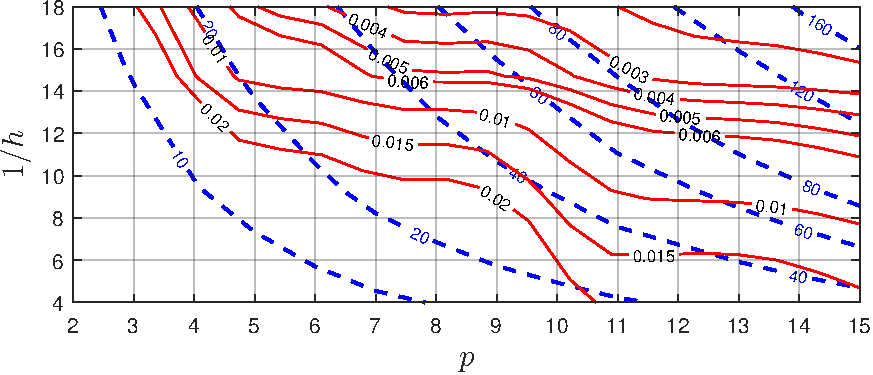
\includegraphics[width=\linewidth, height=4cm]{figs/hp_str-tri.pdf} 
        \caption{structured triangular mesh}
        \label{hp_str-tri}
    \end{subfigure}
    %\hfill
    \begin{subfigure}[t]{0.45\textwidth}
        \centering
        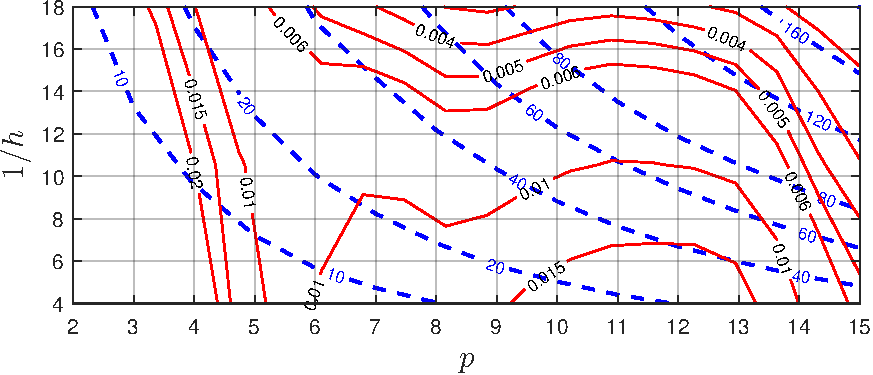
\includegraphics[width=\linewidth, height=4cm]{figs/hp_unstr-tri.pdf}  
        \caption{unstructured triangular mesh}
        \label{hp_unstr-tri}
    \end{subfigure}

    \caption{Contour plots showing the runtime (blue dotted line) in seconds and error (red solid line) in conduction speed relative to the true speed in solving the monodomain equation for each $hp$ combination using three types of mesh.}
    \label{hp}
\end{figure}

The optimal $hp$ combination was defined as the one that gives the shortest runtime for a desired level of error. Figure \ref{hp} can be used as a reference for selecting the optimal discretisation. The inverse of $h$ on the y-axis effectively reflects the number of elements generated. In general, increasing the polynomial order above 6 yields a reduced effect on improving the accuracy. This is particularly evident when the number of elements is high (around $1/h = 18$), where increasing the polynomial order becomes more effective than refining the mesh.  This trend holds true for all three types of mesh used. Additionally, some error contours do not intersect the x-axis, indicating a minimum element size required to achieve certain levels of accuracy. For example, achieving an error smaller than 0.6\% using structured quadrilateral mesh requires an element size smaller than 1/7. The structured triangular mesh reaches errors below 0.3\% more efficiently than the other two types in this specific example. Runtime remained consistent across mesh types. It should be noted that the data in Figure \ref{hp} has been filtered and interpolated to highlight general trends more clearly. While minimal filtering and interpolation were applied consistently, it is possible that individual cases may deviate significantly from the observed trend, such as the singular case at around $p = 5$ and $1/h$ between 4 and 12 with unstructured triangular mesh. This case deviates from the trend observed in the structured meshes and was not filtered out. Also, with quadrilateral and unstructured triangular mesh, there is a sharp increase in accuracy from $p = 14$ to $p = 15$. This suggests that the simulation may be sensitive to the polynomial order such that the accuracy is much higher at some specific orders.  

\subsection{Changing conductivity and cell membrane capacitance}
\begin{figure}[ht!]
    \centering
    
    \begin{subfigure}{0.45\textwidth}
        \centering
        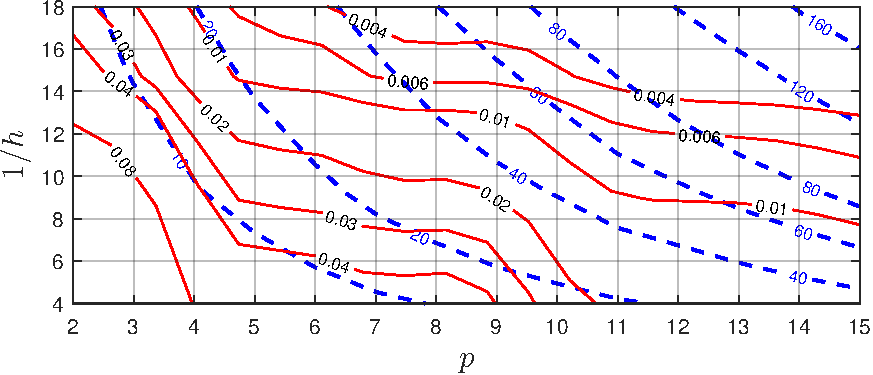
\includegraphics[width=\linewidth, height=4cm]{figs/cond1.00.pdf}  
        \caption{$\sigma = 1.00$, $C_m = 0.0100$}
        \label{cond1.00}
    \end{subfigure}
    %\hfill
    \begin{subfigure}{0.45\textwidth}
        \centering
        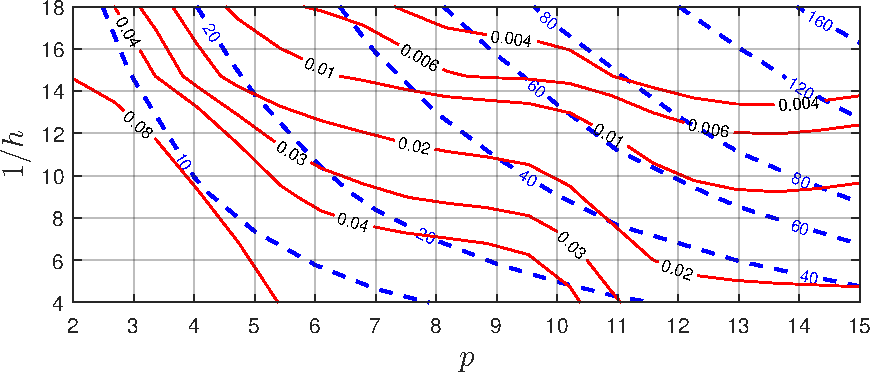
\includegraphics[width=\linewidth, height=4cm]{figs/cond0.75.pdf} 
        \caption{$\sigma = 0.75$, $C_m = 0.0100$}
        \label{cond0.75}
    \end{subfigure}
    %\vspace{1em}  % vertical space between rows
    \begin{subfigure}{0.45\textwidth}
        \centering
        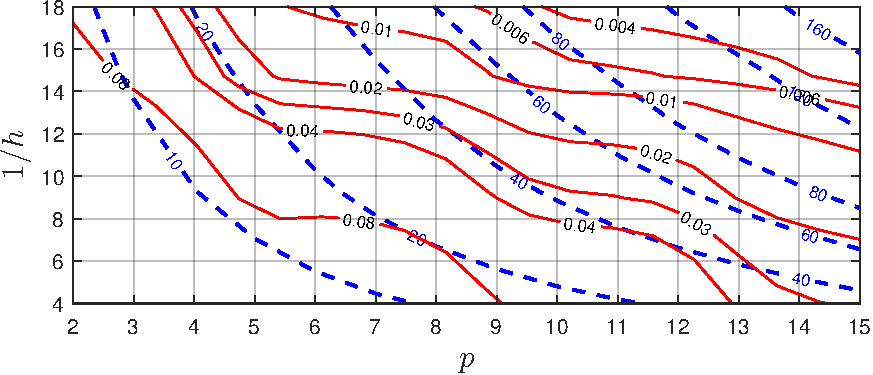
\includegraphics[width=\linewidth, height=4cm]{figs/cond0.50.pdf}  
        \caption{$\sigma = 0.50$, $C_m = 0.0100$}
        \label{cond0.50}
    \end{subfigure}
    %\hfill
    \begin{subfigure}{0.45\textwidth}
        \centering
        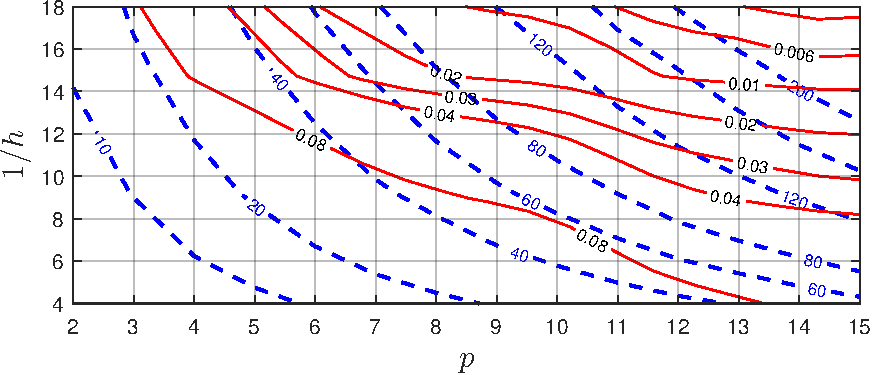
\includegraphics[width=\linewidth, height=4cm]{figs/cond0.25.pdf}  
        \caption{$\sigma = 0.25$, $C_m = 0.0100$}
        \label{cond0.25}
    \end{subfigure}
    \begin{subfigure}{0.45\textwidth}
        \centering
        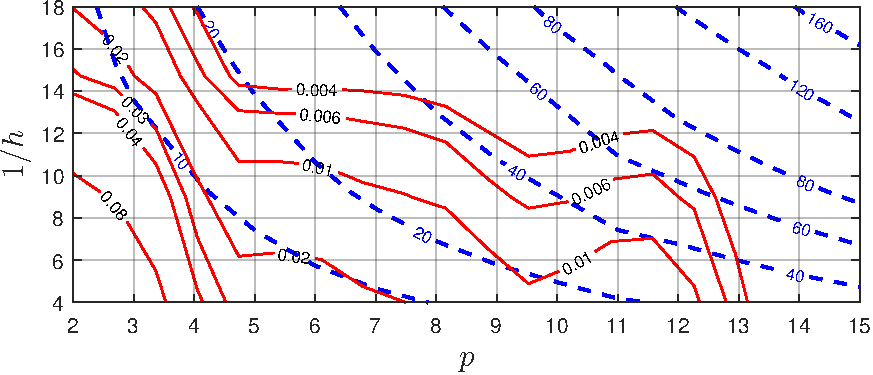
\includegraphics[width=\linewidth, height=4cm]{figs/cm0.0050.pdf} 
        \caption{$\sigma = 0.10$, $C_m = 0.0050$}
        \label{cm0.0050}
    \end{subfigure}
    \begin{subfigure}{0.45\textwidth}
        \centering
        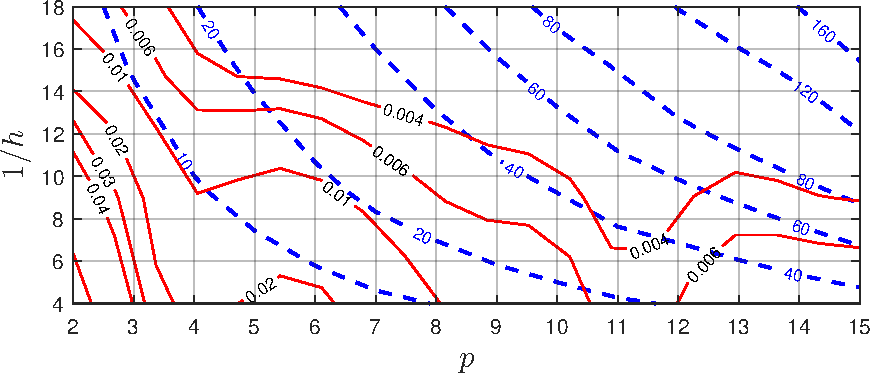
\includegraphics[width=\linewidth, height=4cm]{figs/cm0.0025.pdf}  
        \caption{$\sigma = 0.10$, $C_m = 0.0025$}
        \label{cm0.0025}
    \end{subfigure}
    \caption{Contour plots showing the runtime (blue dotted line) in seconds and error (red solid line) in conduction speed relative to the true speed in solving the monodomain equation for each $hp$ combination using structured triangular mesh with different coefficients of $\sigma$ and coefficients of membrane capacitance $C_m$.}
    \label{coeff}
\end{figure}
In summary, both decreasing the conductivity and increasing the membrane capacitance can increase the error without affecting runtime. The effects of these parameters can be understood by inspecting Equation \ref{monodomain}. 
\par
Figure \ref{coeff} compares the error and runtime for each $hp$ combination using structured triangular mesh with different $\sigma$ and $C_m$. Notice that all the plots in Figure \ref{coeff} have the same values of errors and runtime plotted. Figures \ref{cond1.00} to \ref{cond0.25} show that decreasing the conductivity generally pushes the error contours further up and to the right but preserves their shapes, with the runtime contours being the same. A similar trend can be observed with increasing values of the membrane capacitance as shown in Figures \ref{cond1.00}, \ref{cm0.0050} and \ref{cm0.0025}. As with the previous section, the error plots have been filtered and interpolated to emphasize overall trends rather than specific $hp$ combinations.

\subsection{Comparison of quadrature point distribution}
\begin{figure}[h!]
    \centering

    \begin{subfigure}{0.45\textwidth}
        \centering
        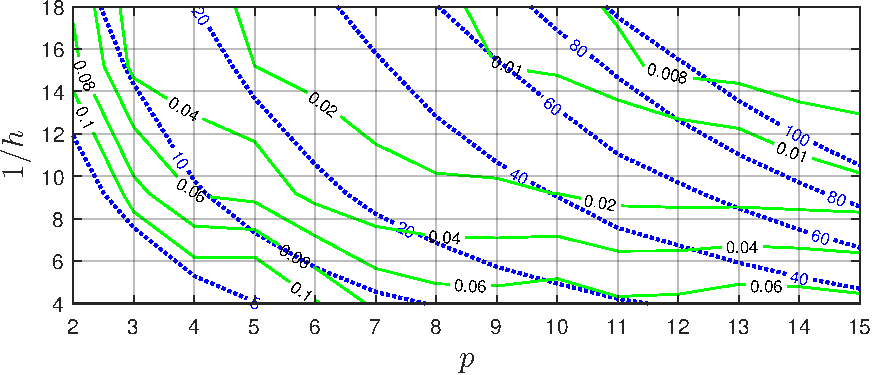
\includegraphics[width=\linewidth, height=4cm]{figs/distri_str_origin_std.pdf}  
        \caption{Structured triangular mesh, Gaussian distribution}
        \label{distri_str_origin_std}
    \end{subfigure}
    %\hfill
    \begin{subfigure}{0.45\textwidth}
        \centering
        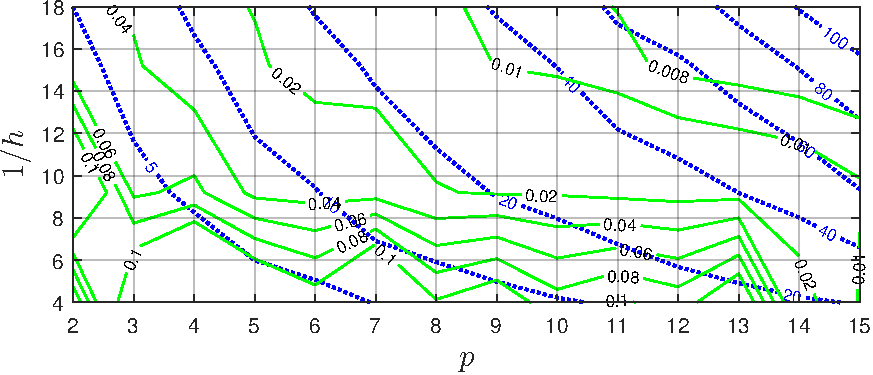
\includegraphics[width=\linewidth, height=4cm]{figs/distri_str_nodal_std.pdf}  
        \caption{Structured triangular mesh, Nodal distribution}
        \label{distri_str_nodal_std}
    \end{subfigure}

    \begin{subfigure}{0.45\textwidth}
        \centering
        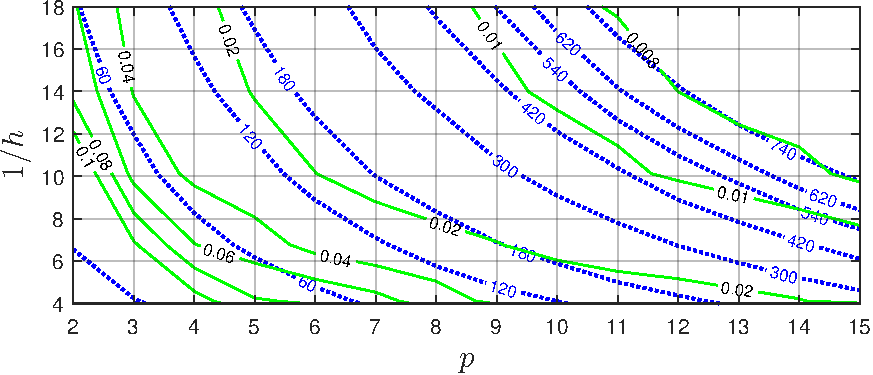
\includegraphics[width=\linewidth, height=4cm]{figs/distri_unstr_origin_std.pdf}  
        \caption{Unstructured triangular mesh, Gaussian distribution}
        \label{distri_unstr_origin_std}
    \end{subfigure}
    %\hfill
    \begin{subfigure}{0.45\textwidth}
        \centering
        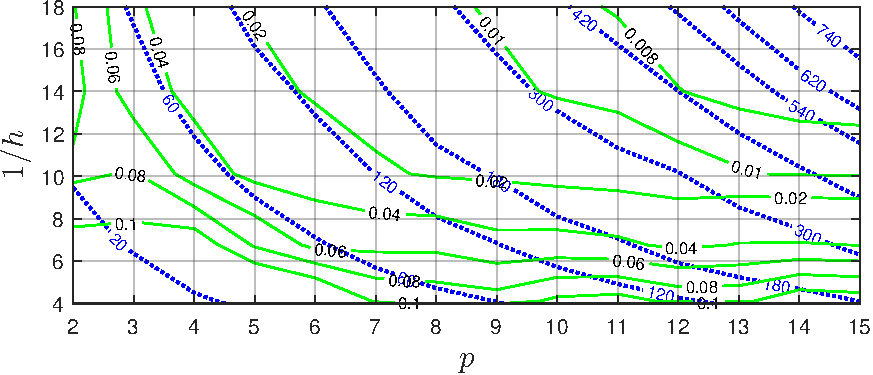
\includegraphics[width=\linewidth, height=4cm]{figs/distri_unstr_nodal_std.pdf} 
        \caption{Unstructured triangular mesh, Nodal distribution}
        \label{distri_unstr_nodal_std}
    \end{subfigure}
    
    \caption{Contour plots showing the runtime (blue dotted line) in seconds and the standard deviation (green line) of the x-coordinates of the wavefront in solving the monodomain equation for each $hp$ combination using structured and unstructured triangular mesh with Gaussian and Nodal point distributions used in the cell model.}
    \label{distri_str}
\end{figure}
Switching from Gaussian to nodal quadrature points significantly reduces runtime, as expected, since nodal distribution uses fewer quadrature points. However, this comes at the cost of reduced solution quality, particularly in terms of capturing the uniformity of the wavefront. Figures \ref{distri_str_origin_std} and \ref{distri_str_nodal_std} show that increasing the polynomial order or the number of elements consistently improves wavefront uniformity for both Gaussian and nodal distributions.
\par
In the case of unstructured triangular mesh, where the domain was enlarged to [0,10][0,5], Figures \ref{distri_unstr_origin_std} and \ref{distri_unstr_nodal_std} reveal that nodal distribution generally results in poorer uniformity compared to Gaussian distribution, except for cases where $h > 700$. For large $h$, both distributions perform similarly. It is also evident that at lower $h$ values, increasing the polynomial order has minimal effect on improving uniformity when using nodal distribution. Nevertheless, using nodal distribution significantly reduces the runtime. Note that Figure \ref{distri_str} was plotted using the original data without being filtered or interpolated. 
